\documentclass[a4paper,12pt]{article}
\usepackage[utf8]{inputenc}
\usepackage{amssymb,amsmath,uniinput,graphicx,hyperref, multirow,units}
\usepackage[section]{placeins}
\usepackage[ngerman]{babel}
\usepackage[left=3cm,right=3cm,top=3cm,bottom=3cm]{geometry}
\renewcommand{\familydefault}{\sfdefault}
\setlength{\belowcaptionskip}{6pt}
\hypersetup{pdfinfo = {
	Title={Versuchsprotokoll zur Paulschen Teilchenfalle},
	Author={Knut Kiesel, Tobias Pook},
	Keywords={Teilchenfalle}
}}


\graphicspath{ {../pictures/} }
\title{Laborpraktikum Teilchenphysik\\ Paulsche Teilchenfalle}
\author{Knut Kiesel\\Tobias Pook}
\date{\today}

\begin{document}
\maketitle
\vspace{5cm}
\tableofcontents
\thispagestyle{empty}
\newpage
\setcounter{page}{1}

\section{Ziel der Messung} % max 1 Seite
Ziel des Versuches ist die Speicherung von elektrisch geladenen Teilchen und die Bestimmung des Verhältnisses von Ladung zu Masse.
Um die Teilchen in einem räumlich begrenzten Feld zu halten, ist ein statisches elektrisches Feld nicht ausreichend, da man damit keine Potentialminima schaffen kann.
Eine Möglichkeit dennoch Teilchen zu fangen ist das Anlegen von phasenverschobenen Wechselspannungen und Gleichspannungen, wobei bei richtiger Einstellungen der Spannungen und Frequenzen die Teilchen stabil in der Falle bleiben.
Konkret wurden beim durchgeführten Experiment der meta-stabile Bereich eines rotierenden Sattelpotential genutzt um Teilchen zu speichern.
Für jede räumliche Komponente $i\in\{x,y,z\}$ lautet die Bewegungsgleichung
\begin{align}\label{mastergleichung}
	\frac{4}{mΩ^2} |\vec{F}_i| + \left( a_i -2q_i \cos\left( 2\xi_i \right) \right) i  + 2k_L \frac{dx}{d\xi_i} + \frac{d^2x}{d\xi_i^2} = B\cos\left( \frac{2ω_W}{Ω}ξ_i \right)
\end{align}
mit dem gleichstromabhängigen Koeffizienten $a_i = \frac{16KqU_{G,i}}{3Ω^2mr_0^2}$,
dem wechselstromabhängigen Koeffizienten  $q_i = -\frac{4kqU_i}{Ω^2mr_0^2}$,
dem Antribskoeffienzenten $B = \frac{2qU_W}{r_0mΩ^2}$,
dem Luftreibungskoeffizient $k_L = \frac{6πηR}{mΩ}$, der Winkelfrequenz der Dreiphasenspannung $Ω$,
der Winkelfrequenz der zusätzlich an einem Plattenpaar angelegten Wechselspannung $ω_W$
und der normalisierten Zeit $ξ_i = \frac{Ωt}{2} + \frac{iπ}{3}$.
$\vec{F}$ ist eine konstante äußere Kraft, zum Beispiel bei der z-Komponente die Gewichtskraft.
Die Grundschwingung der Lösung wird durch
$$β_i = \sqrt{a_i + \frac{q_i^2}{2}}$$
beschrieben.
Durch Anlegen geeigneter Frequenzen und Spannungen und das Beobachten der entstehenden Teilchenbewegungen kann mit unterschiedlichen Methoden das Verhältnis von Ladung zur Masse bestimmt werden.


\section{Aufbau und Durchführung}
Die z-Achse verläuft vertikal, die y-Achse ist die Blickrichtung, und die x-Achse liegt senkrecht zu den beiden übrigen.

Die Falle wird aus sechs Kupferringen und 12 Verbindungsstücken zu einem Würfel geklebt.
Nach dem Anlöten und Isolieren der Anschlusskabel wird die Falle mit schwarzem Lack angestrichen, um Steulicht in der Kammer zu verringern.
Die Falle wird mittig über der Öffnung für die Spritze an den Anschlusskabeln befestigt und die Plattform von unten an die Spannungsversorgung angeschlossen (siehe Abbildung \ref{fallenbild}),
welche je nach Hebelstellung die Gleichspannungen oder die zusätzliche Wechselspannung zur Dreiphasenspannung hinzufügt.
Die Dreiphasenspannung, im folgenden auch Fokussierspannung genannt, wird aus drei Wechselpannungsquellen die mit einem konstanten Phasenunterschied von $120^\circ$ betrieben werden, geliefert (siehe Abbildung \ref{verschaltung3phase}).
Die Amplitude kann dabei für jedes Flächenpaar individuell eingestellt werden.

\begin{figure}[htb]
		\centering
		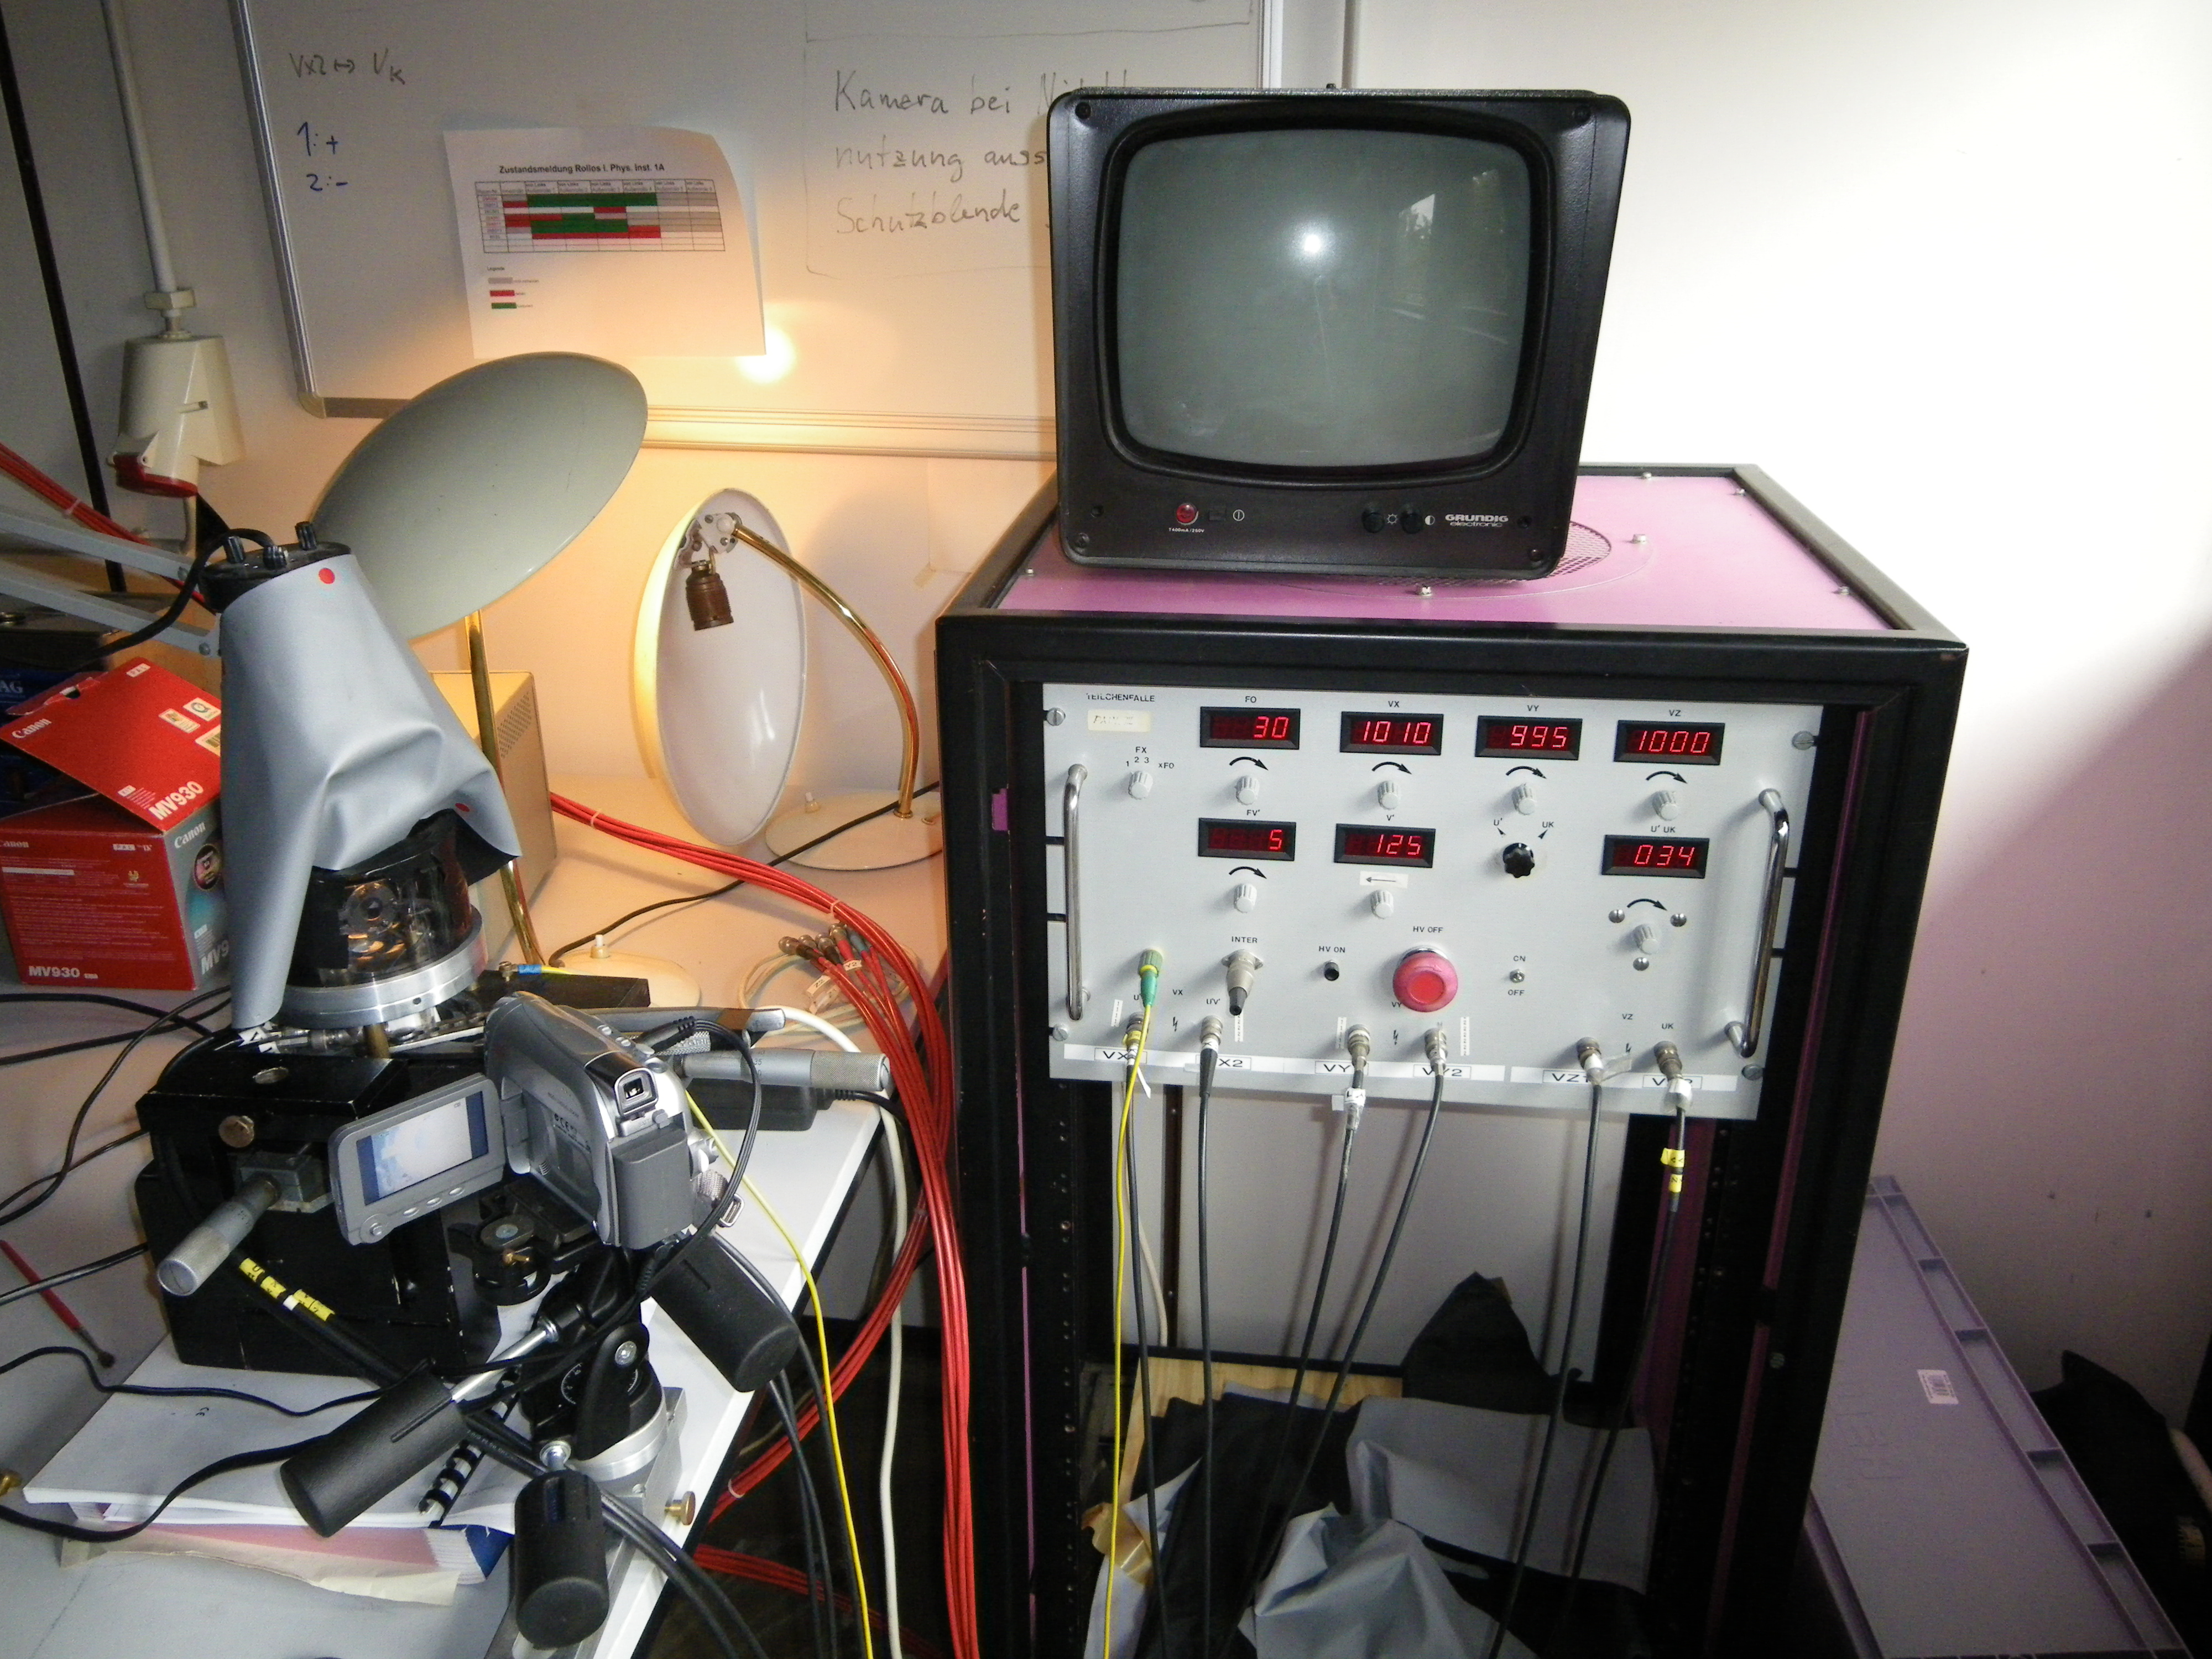
\includegraphics[width=0.8\textwidth]{aufbau.jpg}
		\caption{Versuchsaufbau der Paulschen Teilchenfalle}
		\label{fallenbild}
\end{figure}

Es gibt mehrere Möglichkeiten die Gleichspannung anzulegen:
Man kann sie auf den beiden gegenüber liegenden Seiten (siehe Abbildung \ref{verschaltungstab}) oder zwischen zwei
gegenüberliegenden Seiten (siehe Abbildung \ref{verschaltungz}) anbringen.
Die Wechselspannung wird zwischen zwei gegenüberliegenden Flächen angelegt (siehe Abbildung \ref{verschaltungres}), Frequenz und Amplitude sind einzeln regelbar.
Die Verschaltung ist jedoch schon vorgefertigt und kann mit Schaltern hinzugeschaltet werden.

\begin{figure}[htb]
		\centering
		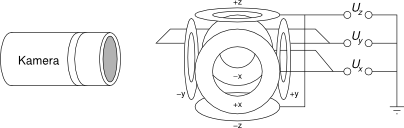
\includegraphics{Schaltbild_3Phasen.png}
		\caption{Verschaltung im Generator für die Fokussierspannung}
		\label{verschaltung3phase}
\end{figure}

\begin{figure}[htb]
		\centering
		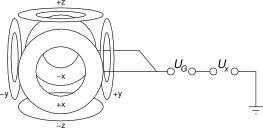
\includegraphics{Schaltbild_Stabilitaet.png}
		\caption{Verschaltung im Generator für eine Gleichspannung auf zwei Flächen}
		\label{verschaltungstab}
\end{figure}

\begin{figure}[htb]
		\centering
		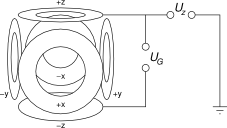
\includegraphics{Schaltbild_Z_Kompensation.png}
		\caption{Verschaltung im Generator für die Gleichspannung zwischen zwei Flächen}
		\label{verschaltungz}
\end{figure}

\begin{figure}[htb]
		\centering
		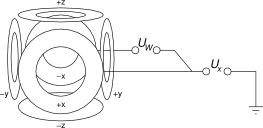
\includegraphics{Schaltbild_Wechselspannung.png}
		\caption{Verschaltung im Generator für die Wechselspannung zwischen zwei Flächen}
		\label{verschaltungres}
\end{figure}
Aus Sicherheitsgründen wird die Falle durch eine durchsichtige Acrylhaube abgedeckt.
Die Haube wurde zusätzlich mit Ausnahme von zwei Stellen mit schwarzem Klebeband verkleidet.
Die zwei Öffnungen dienen der seitlichen Beobachtung der Falle und der Bestrahlung durch eine oben angebrachten Lampe.
Die geladen Teilchen sind Aluminiumpulverstücke, die mittels einer Spritze durch eine Öffnung unterhalb der Falle eingebracht werden.
Durch das Reiben an der Spritzenöffnung werden die Aluminiumteile ionisiert.
Da zwischen Öffnung und dem stabilen Bereich der Teilchenfalle ein Abstand von ca. $\unit[2.5]{cm}$  besteht wurden die Teilchen durch anschnipsen der Spritze in die Falle geschleudert.
Zusätzlich zum Messaufbau in Luft gibt es noch einen zweiten Messaufbau für Versuche im Vakuum. Hier befindet sich eine baugleiche Falle in einer zylindrischen Vakuumkammer.
Die Kammer besitzt mehrere Öffnungen an denen Beobachtungsfenster,Stromversorgung,Vakuumpumpe und ein beweglicher Hebel mit Halterung für die Spritze druckdicht angebracht werden können.
 Da während der Versuchsdurchführung die Vakuumpumpe defekt war 
konnten Messungen lediglich bei vermindertem Luftdruck, im Bereich zwischen $\unit[300]{mbar} - \unit[450]{mbar}$, durchgeführt werden.  

Es gibt auch eine vorgefertigte Falle, die sich in einer Vakuumkammer befindet.
Diese kann man mit einem einer normalen Turbinenpumpe und bei niedrigeren Drücken mit einer Turbo-Molekularpumpe vakuumisieren und den Druck mithilfe eines Drucksensors überprüfen.
Durch Scheiben kann man die Falle ebenso anleuchten und beobachten.



\section{Ergebnisse}
Mit einem Messschieber wird der Plattenabstand der Teilchenfalle auf $d = \unit[(3.05±0.02)]{cm}$ abgeschätzt.
\subsection{Bahnbeschreibung}
In den meisten Fällen beschreiben die eingefangenen Teilchen eine elliptische Teilchenbahn deren Radius und die Exzentrizität durch das Verhältnis der angelegten Potenziale in der Fokusierspannung erklärt werden können.
Viele Teilchen beschreiben zudem sehr kleine Bahnen und sind deshalb nur noch als Punkte wahrzunehmen.

\subsubsection*{Lissajous Figuren}
Manchmal bilden sich auch Lissajou Figuren. Lissajous Figuren entstehen bei der Überlagerung harmonischer Schwingungen, wenn das Verhältnis der Frequenzen rational ist.
In diesem Fall bildet die Teilchenbahn eine geschlossene Figur.
Die möglichen Formen der Figuren sind sehr vielfältig und hängen vom Frequenzverhältnis und dem Phasenunterschied der Schwingungen ab.
Ein Beispiel ist in Abbildung \ref{Lissjous} zu sehen.

\begin{figure}[htb]
		\centering
		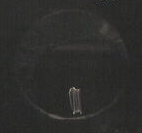
\includegraphics{lisa_klein.jpg}
		\caption{Beispiel für das auftreten einer Lissajous Figur}
		\label{Lissjous}
\end{figure}

\subsubsection*{Kristallstruktur}
Wenn man mehrere Teilchen in der Teilchenfalle gefangen hat, kann man manchmal pseudo Kristallstrukturen erkennen:
Die Teilchen stoßen sich gegenseitig ab und suchen energetisch günstige Zustände, ebenso wie in einem Kristall.
Überlagert zu diesem Effekt sieht man in Abbildung \ref{pseudokristall} noch die Auswirkungen des Feldes.
In der hier sichtbaren $x = 0$ und $z = 0$ Ebene werden keine Teilchen gehalten, wie man auch Gleichung (\ref{mastergleichung}) entnehmen kann.

\begin{figure}[htb]
		\centering
		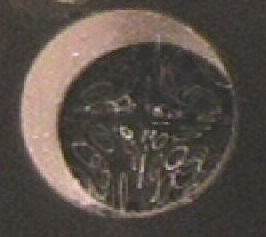
\includegraphics{pseudo_kristall.png}
		\caption{Beispiel zur Pseudokristallstruktur}
		\label{pseudokristall}
\end{figure}

\subsubsection*{Fangen von Teilchen im Vakuum}
Beim vakuumisieren der Kammer kann der gewünschte Druck von einigen $\unit{μbar}$ erreicht werden.
Die Frontanzeige liefert bei Erreichen von $90μbar$ auf einen Fehlercode und auch auf der Rückseite des Sensors ist der Druck immer noch zu groß.
Auch das Halten von Teilchen in der Falle gestaltet sich bei diesen Einstellungen noch als schwierig, man kann erahnen wie die Teilchen immer zu einer Seite abgesaugt werden.
Grund dafür könnte ein Leck an der Vakuumskammer sein, ein defekt der Turbo-Molekularpumpe ist aber auch nicht ausgeschlossen.
Da das Saugen der Pumpe jede Speicherung während des Pumpens unmöglich macht, ist die eingize Möglichkeit, Teilchen in der Vakuumfalle zu halten, die Pumpe auszuschalten.
Der Druck fällt rasch auf ein paar $\unit[100] {mbar}$ ab und ist dann relativ stabil, was einem das einfangen von Teichen erlaubt.


\subsection{Kompensation der Gewichtskraft}
In Gleichung (\ref{mastergleichung}) wird der Einfluss der Luftreibung vernachlässigt und ein Näherungsansatz der Form $z(ξ_z) = Z(ξ_z)+d(ξ_z)$ durchgeführt.
Die z-Komponente wird nun durch
\begin{align*}
	Z(ξ) = Z_0\sin(β_zξ) - \frac{4|\vec{F}_z|}{mβ_zΩ^2}
\end{align*}
beschrieben.
Man sieht, dass die Schwingung um einen konstanten Term verschoben ist, der von $a_z$ und $q_z$ abhängt.
Diese Abhängigkeit besteht nicht mehr, wenn gilt:
\begin{align}
	\label{kraftgleichgew}
	|\vec{F}_{z}| = |\vec{F}_G + \vec{F}_{qE}| = mg + q\frac{U_G}{d} = 0
\end{align}

Zu der Dreiphasenspannung wird nun ein zusätzlicher Potentialunterschied zwischen den beiden z-Komponenten angeschlossen (siehe Abbildung \ref{verschaltungz}), der solange erhöht wird, bis die Gravitationskraft kompensiert wird.
Dies kann dadurch überprüft werden, dass sich der Mittelpunkt der Teilchenschwingung bei Änderung der Amplitude der z-Komponente der Dreiphasenspannung nicht mehr ändert.
Die Fokussierspannung wird bei $U_i = \unit[(1000±50)]{V}$ für alle Flächenpaare betrieben.


Weil die Gleichspannung stark schwankend ist, wird die effektive Spannung durch notieren der angezeigten Werte in einem Zeitraum von ungefähr $\unit[20]{s}$ und anschliessendem Mitteln bestimmt. 
Der Fehler auf die Stichprobe wird im folgenden als statistischer Fehler angenommen.
Da man die Teilchen oft wegen spontaner Spannugsschwankungen der Quelle verliert, kann der Bereich in dem die Gravitationskraft kompensiert wird, nicht in feineren Spannungsabschnitten untersucht werden.
Dies führt dazu, dass nicht abgeschätzt werden kann wie exakt der Wert für die Kompensationsspannung $U_G$ getroffen wird.
Die mittlere Differenz zu den nächstliegenden $U_G$ Messwerten, bei denen wieder Bewegungen des Schwingungsmittelpunkt bei Variation der Fokussierspannung $U_z$ zu beobachten sind,
wird deshalb als systematischer Fehler angenommen.
Die Messungen werden teilweise für mehrere gleichzeitig gefangene Teilchen durchgeführt und die Spannung erhöht bis alle Teilchen den Stabilitätsbereich verlassen haben. Die Messergebnisse sind in
Tabelle \ref{tab:z-komp-measure} aufgeführt, dabei werden für die einzelnen Messungen unterschiedliche Teilchen benutzt. Es wurde zusätzlich eine Messung unter vermindertem Luftdruck von
 \unit[(450±50)]{mbar} durchgeführt.
Das Vorzeichen der Ladung ergibt sich aus dem Anschluss an die Spannungsquelle und ist für alle beobachteten Teilchen negativ, was mit der Theorie übereinstimmt.

\begin{table}
	\centering
	\begin{tabular}{ l | c | l | l }
		$U_{G} [V]$ & $\sigma_{U_{G}}[V]$ & \multicolumn{2}{l}{Verhalten des Bahnmittelpunkts bei Änderung von $U_z$}  \\
		\hline
		\hline
		Messung 1 (2 Teilchen)& & &\\
		\hline
		45 & 5 & Bewegung &  Bewegung   \\
		92 & 8 & still  & Bewegung \\
		168 & 4 & Bewegung & Bewegung    \\
		228 & 3 & Bewegung & Bewegung \\
		273 & 5 & verloren & still \\
		\hline
		\hline
		Messung 2 (1 Teilchen) & & &\\
		\hline
		33 & 5 & Bewegung \\
		50 & 4 & still\\
		60 & 5 & Bewegung \\
		79 & 7 & Bewegung\\
		\hline\hline
		Messung $3^*$ (1 Teilchen)& & &\\
		\hline
>>>>>>>>>>>>>>>>>>>> File 1
		Messung 3 (1 Teilchen)& & &\\
		verminderter Luftdruck & & &\\
	    $p = \unit[(450±50)]{mbar}$ & & &\\
>>>>>>>>>>>>>>>>>>>> File 2
		Messung 3 (1 Teilchen)& & &\\
		verminderter Luftdruck & & &\\
	    $p = \unit[(450±50)]{mbar}$ & & &\\
>>>>>>>>>>>>>>>>>>>> File 3
<<<<<<<<<<<<<<<<<<<<
		25 & 3 & Bewegung\\
		68 & 3 & still\\
		79 & 7 & Bewegung\\
	\end{tabular}
	\caption{Verhalten von beiden Teilchen bei unterschiedlichen Gleichspannungen zur Bestimmung der z-Kompensation.\newline
		* Messung 3 wurde unter vermindertem Luftdruck von $p = \unit[(450±50)]{mbar}$ durchgeführt.
	}
	\label{tab:z-komp-measure}
\end{table}

Aus Gleichung \ref{kraftgleichgew} lässt sich direkt eine Formel für die spezifische Ladung des untersuchten Teilchen herleiten:
\begin{align}\label{zspezm}
	\frac{q}{m} = -\frac{g \cdot  d}{U_{G}}
\end{align}
Die berechneten Werte können Tabelle \ref{tab:z-komp-result} entnommen werden. Hierbei wird die Erdbeschleunigung 
$g = \unitfrac[(9.81)]{m}{s}$ als fehlerfrei angenommen und die Unsicherheit auf den Fallendurchmesser als weitere
unabhängige systematische Fehlerquelle betrachtet.


\begin{table}
	\centering
	\begin{tabular}{ c | c }
		$\mathbf{U_{G,komp} [V]} $& $\mathbf{\frac{q}{m}[\frac{mC}{kg}]}$ \\
		\hline
		  68 ± 3(stat.) ±27(sys.) &  4.40 ± 0.16(stat.) ± 1.76(sys)  \\
		  50 ± 4(stat.) ±14(sys.) &  5.95 ± 0.53(stat.) ± 1.67(sys)  \\
		  92 ± 8(stat.) ±62(sys.) &  3.27 ± 0.28(stat.) ± 2.21(sys)  \\
		  273 ± 5(stat.) ±55(sys.) & 1.09 ± 0.02(stat.) ± 0.23(sys)  \\
	\end{tabular}
\caption{Das Verhältnis von Ladung zu Masse von verschiedenen Teichen, bestimmt durch die Kompensation der Gewichtskraft}
\label{tab:z-komp-result}
\end{table}

Alle Messwerte liegen in einem mit einander kompatiblen Wertebereich. Durch die hohen systematischen Unsicherheiten auf das 
Treffen der richtigen Kompensationsspannung entstehen relative Unsicherheiten im Bereich von $20\% - 70 \%$. Die erzeugten
Ergebnisse bieten also nur die Möglichkeit grob die Größenordnung der spezifischen Ladungen von Teilchen zu bestimmen.  

\subsection{Resonanz}
In diesem Versuchsteil wird zusätzlich zur Fokusierspannung eine Wechselspannung zwischen dem Flächenpaar entlang der x-Achse angelegt.
Die Gleichspannung wird auf $0$ geregelt.

Bei einer Frequenz von
\begin{align}\label{w_res}
	\omega^{res}_W = \frac{\Omega}{2}\sqrt{\beta^{2}_x-2k^{2}_L}
\end{align}
tritt eine resonante Verstärkung der Oszillation auf und die Teilchenbahn erreicht ihre maximale Auslenkung
\begin{align}\label{Amax}
	A_{max} = \frac{B}{2k_L\sqrt{\beta^{2}_x-k^{2}_L}}.
\end{align}
Durch Eliminieren von $k_L$ in Gleichung \ref{w_res} und \ref{Amax} erhält man
\begin{align}\label{res_luft}
	\frac{q}{m} = ±\sqrt{
		\frac{
			U_w^2r^6Ω^4 ± r^4Ω^2\sqrt{
				(U_wrΩ)^4 - 4(4KU_xA_{max}ω)^4
			} %sqrt
		}{
			128A_{max}^2(KU_x)^4
		} % frac
	}. % sqrt
\end{align}
Für die Lösung im Vakuum reicht es in Gleichung (\ref{w_res}) $k_L=0$ zu setzen, und man erhält
\begin{align}\label{res_vak}
	\frac{q}{m} = -\frac{\Omega r^{2}_0 \omega^{res}_W}{\sqrt{2} K U_x}.
\end{align}

Um die Resonanzfrequenz zu messen, wird die Wechselspannung variiert bis das Teilchen maximale Auslenkung zeigt.
In Luft wird zusätzlich die maximale Amplitude bestimmt, indem mit einer Digitalkamera Fotos der Teilchenbahn angefertigt werden.

Bei niedriger Fokusierfrequenz erhöht sich der relative Fehler und bei hoher Fokusierfrequenz wird die Stabilitätsgrenze schneller erreicht,
darum wurde eine Frequenz von $Ω = (503±6)\unit{Hz}$ und eine Fokusierfrequenz von $\unit[(1414±7)]{V}$ gewählt.
Die Amplitude der Wechselspannung unterliegt starken Schwankungen
( $ \unit[( 210 ± 30 )]{V} $ )
und lässt sich kaum durch den dafür vorgesehenen Drehschalter regeln.
Der Ausschlag der Teilchen wird über das Verhältnis der Amplitude zum Innendurchmesser der Falle $d_{innen}$ bestimmt.
$$A_{max} = \frac{A_{max}\text{ [Pixel]}}{d_{innen}\text{ [Pixel]}} \cdot d_{innen}= \unit[( 0.7 ± 0.4 )]{mm} $$
Alle gemessenen Teilchen zeigen ihre maximale Auslenkung bei $\omega_W < \unit[(31±6)]{Hz}$ ,
dabei handelt es sich um die minimal an der Spannungsquelle einstellbare Frequenz.

Wenn man die Resonanzfrequenz durch die Grundschwingungsfrequenz in Luft $\bar{ω}_0$ ausdrückt, erhalt man
\begin{align*}
	ω^{res}_W = \sqrt{ \bar{ω}_0^2 - \frac{Ω^2k_L^2}{2} },
\end{align*}
was dazu führt, dass die Resonanz unterhalb der Grundschwingungsfrequenz liegt.
Die beobachtete Ereignisse waren wahrscheinlich Schwingungsmaxima, das heißt die eigentlich gesuchte Frequenz liegt unterhalb der Beobachteten.
Um Interpretationsfehler zu vermeiden, wurde dennoch das ganze zur Verfügung gestellte Frequenzspektrum abgefahren, aber ohne eine zusätliche Resonanz zu entdecken.

Auch die Amplitude blieb bei allen drei Teilchen in Luft und drei Teilchen im Vakuum (innerhalb des Fehlers) gleich groß.
Man erhält mit gausscher Fehlerfortplanzung in Luft
$$\frac{q}{m} > \unitfrac[( -0.20 ± 0.20 )]{mC}{kg}$$
und mit der Näherung für Vakuum
$$\frac{q}{m} > \unitfrac[( -0.22 ± 0.05 ) ]{mC}{kg}.$$
Der hohe Fehler bei der genauen Lösung ist durch die Differenzen von hohen Potenzen fehlerbehafteter Größen in Gleichung (\ref{res_luft}) bedingt.
Eine weiterer Grund ist die starke Spannungsschwankung von  $U_w$.
Beide Werte sind untereinander kompatibel, stellen jedoch nur Obergrenzen für das Verhältnisses von Ladung zu Masse dar, da die Resonanzfrequenz nicht weiter regulierbar ist.

%Diese Limitierung der Wechselspanuungsfrequenz in Verbindung mit der stark schwankenden Amplitude
%lassen große Zweifel an der Vertrauenswürdigkeit der gewonnenen Ergebnisse entstehen.

\subsection{Stabilitätsdiagramm}
Wie Gleichung (\ref{mastergleichung}) zu entnehmen, ist die Grundschwingung der Teilchen durch $β$ gegeben.
Wenn $β$ imaginär ist, was äquivalent zu $ a + \frac12q^2 >0$ ist, werden die Winkelfunktionen zu Expotentialfunktionen, was zum Austritt der Teilchen aus der Falle führt.
In diesem Versuchsteil wird explizit nach $β_x = 0$ gesucht.
Dafür wird bei verschiedenen, konstanten $U_x = U_y = U_z = U_i$ die an der x-Achse angelegnent Gleichsannung $U_G$ gesucht, bei der das Teilchen entkommt.
Weil das Teilchen nicht entkommen darf (es muss bei mehreren $U_i$ vermessen werden), ist die Abschätzung nur schwer zu bewerkstelligen, da die Gleichspannungsquelle stark schwankt und es somit leicht entkommen kann.
Für jedes Teilchen wird bei konstantem $Ω =\unit[188±6]{Hz}$ die Gleichspannung $U_g$ gegen $U_i^2$ aufgetragen und eine lineare Regression durchgeführt.
Die Anpassungen sind in Abbildung \ref{linReg} zu sehen.
\begin{figure}[htb]
		\centering
		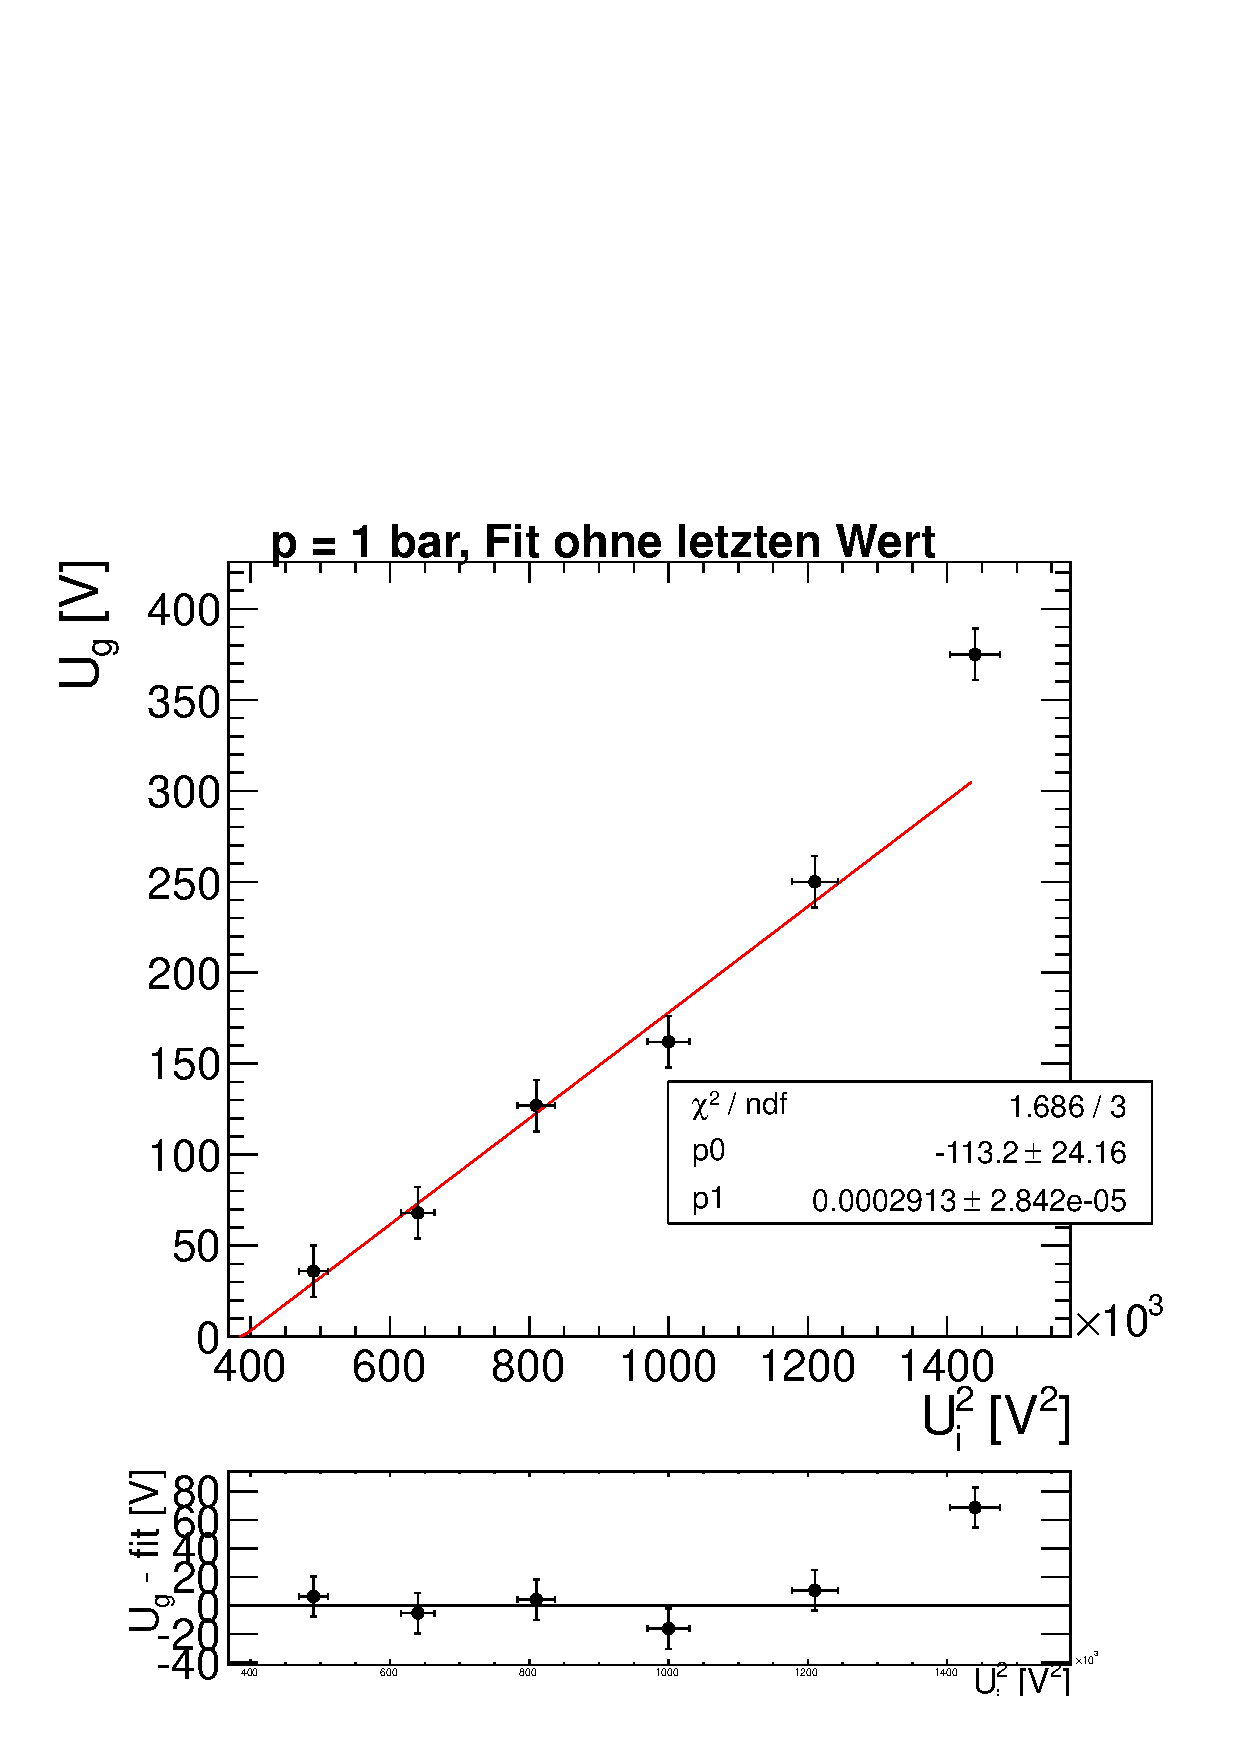
\includegraphics[height = 0.3\textheight]{linRegLuft1.pdf}
		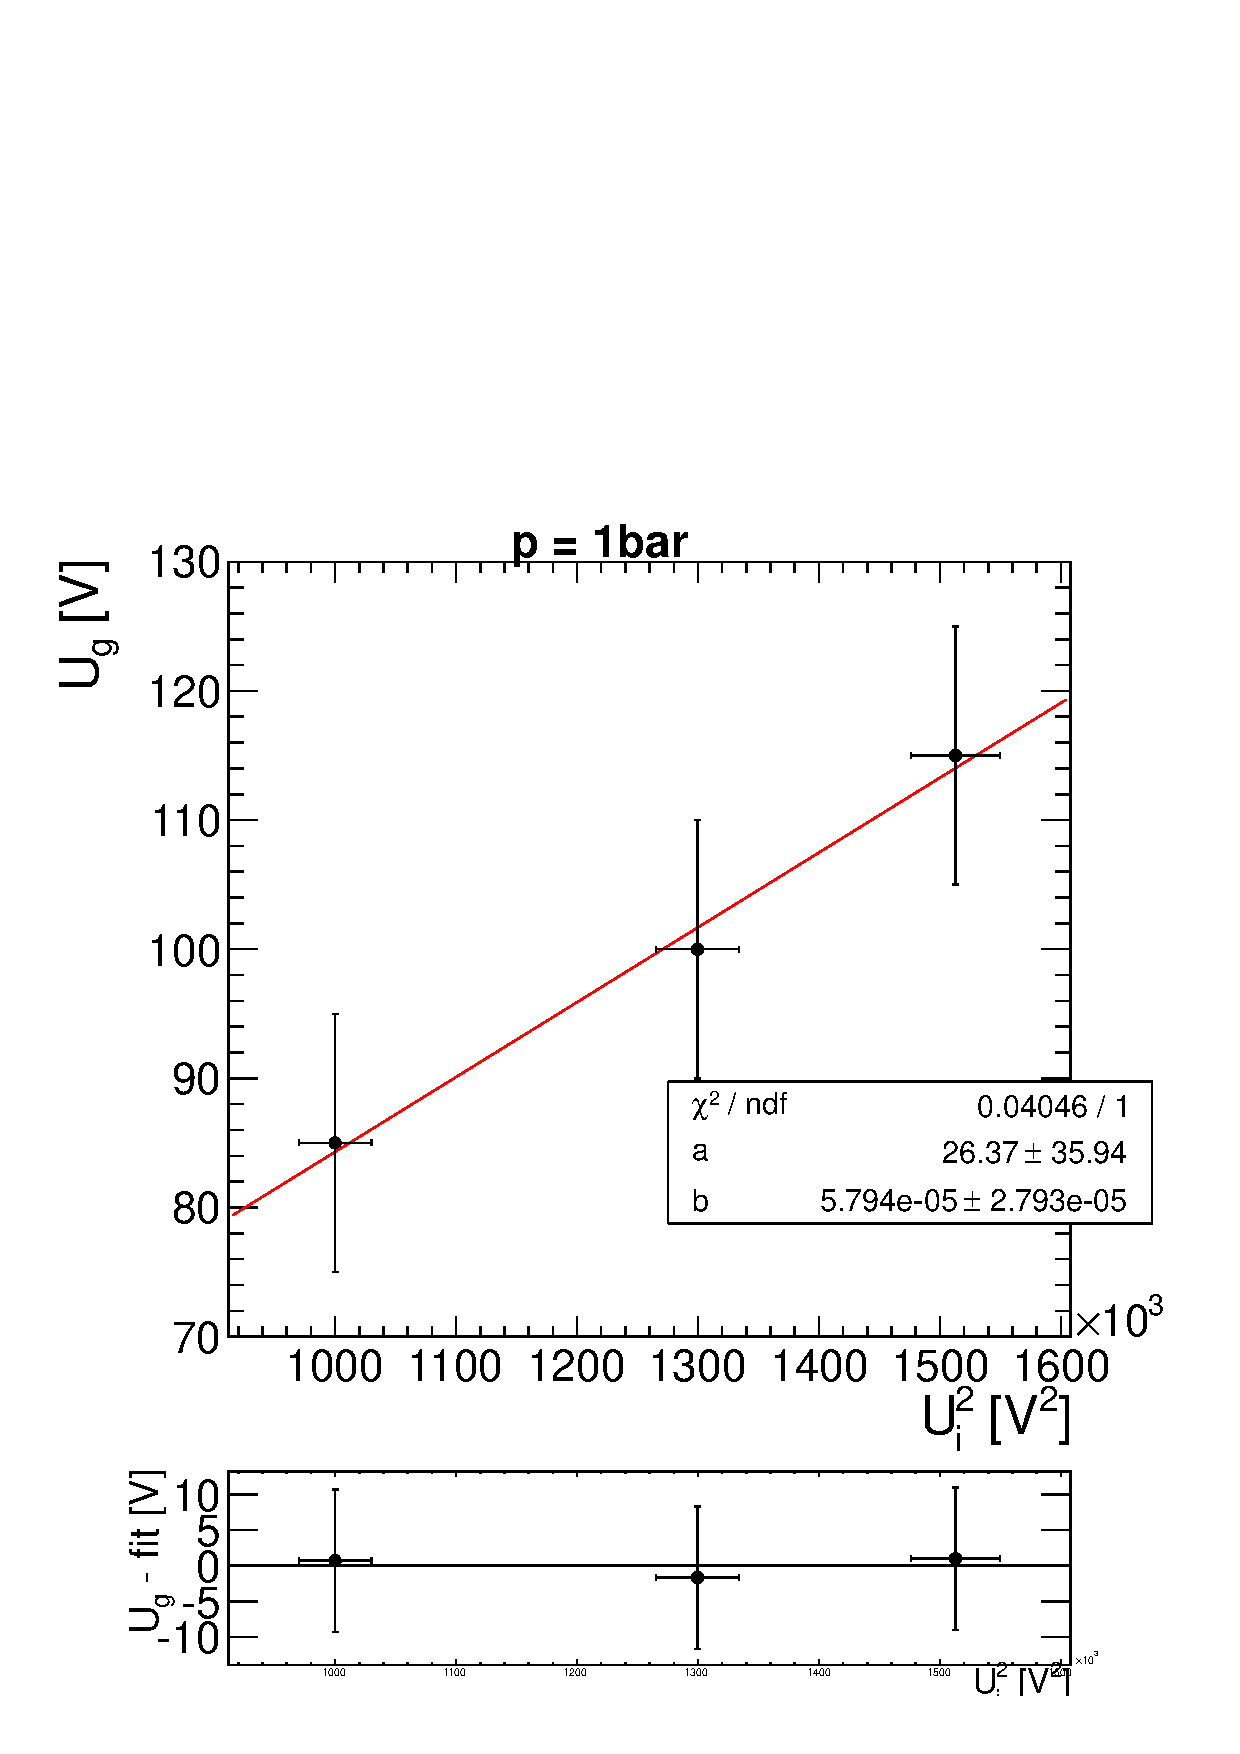
\includegraphics[height = 0.3\textheight]{linRegLuft2.pdf}\\
		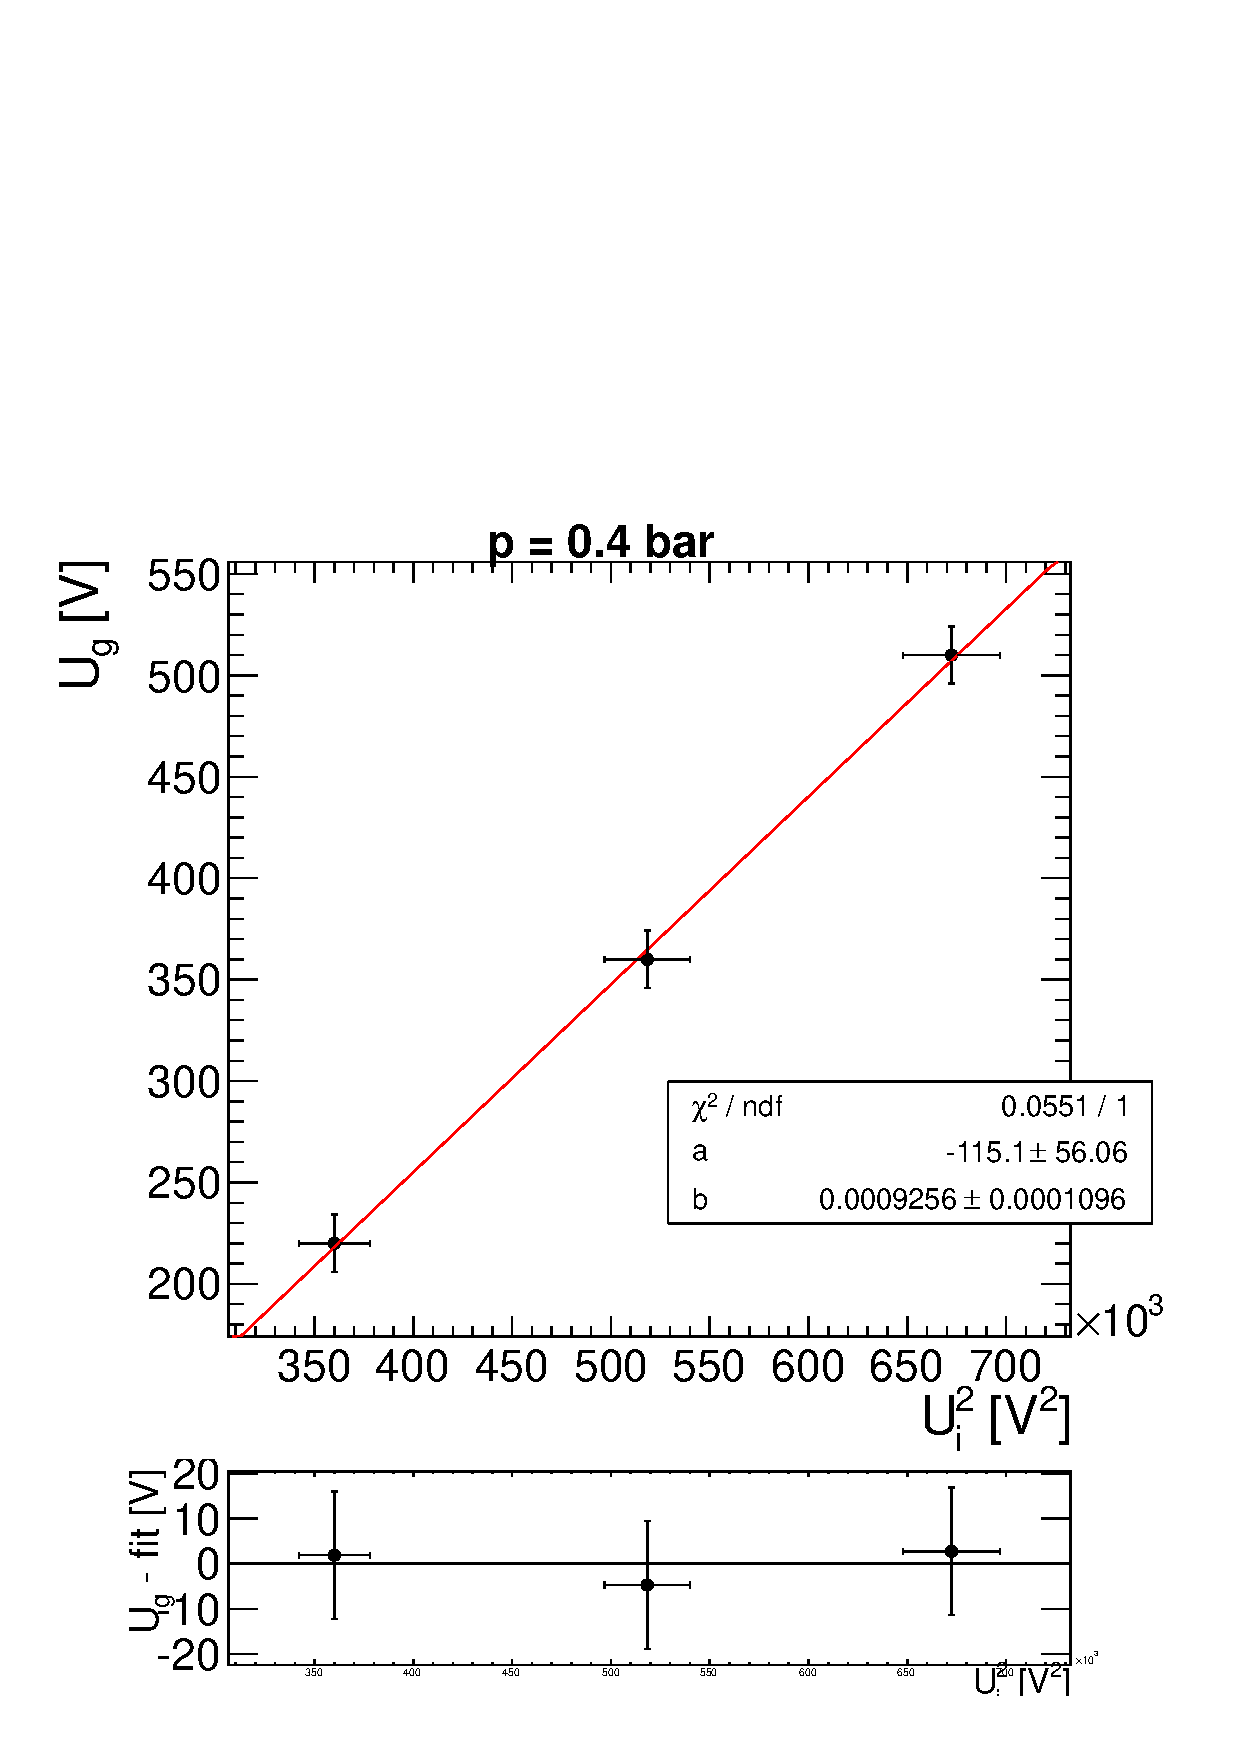
\includegraphics[height = 0.3\textheight]{linReg400bar.pdf}
		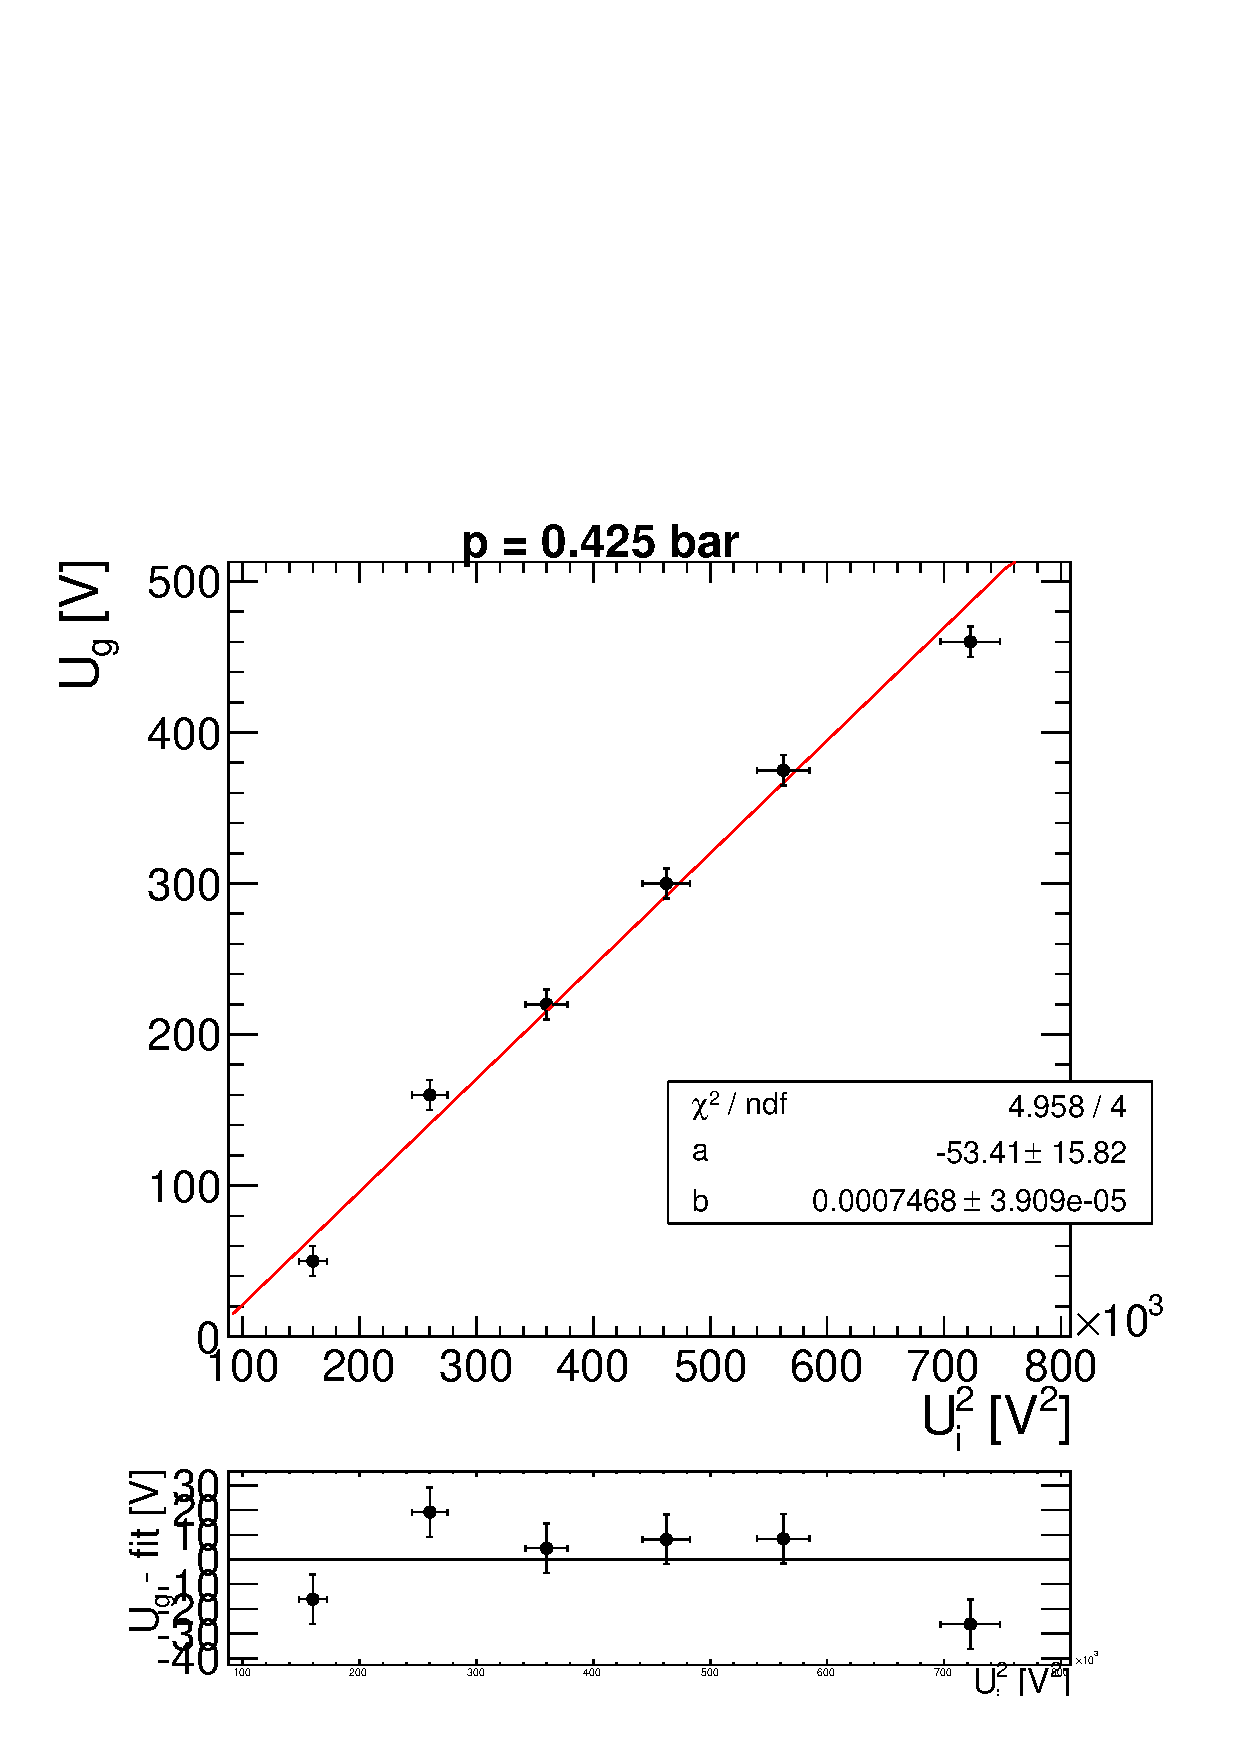
\includegraphics[height = 0.3\textheight]{linReg425bar2.pdf}\\
		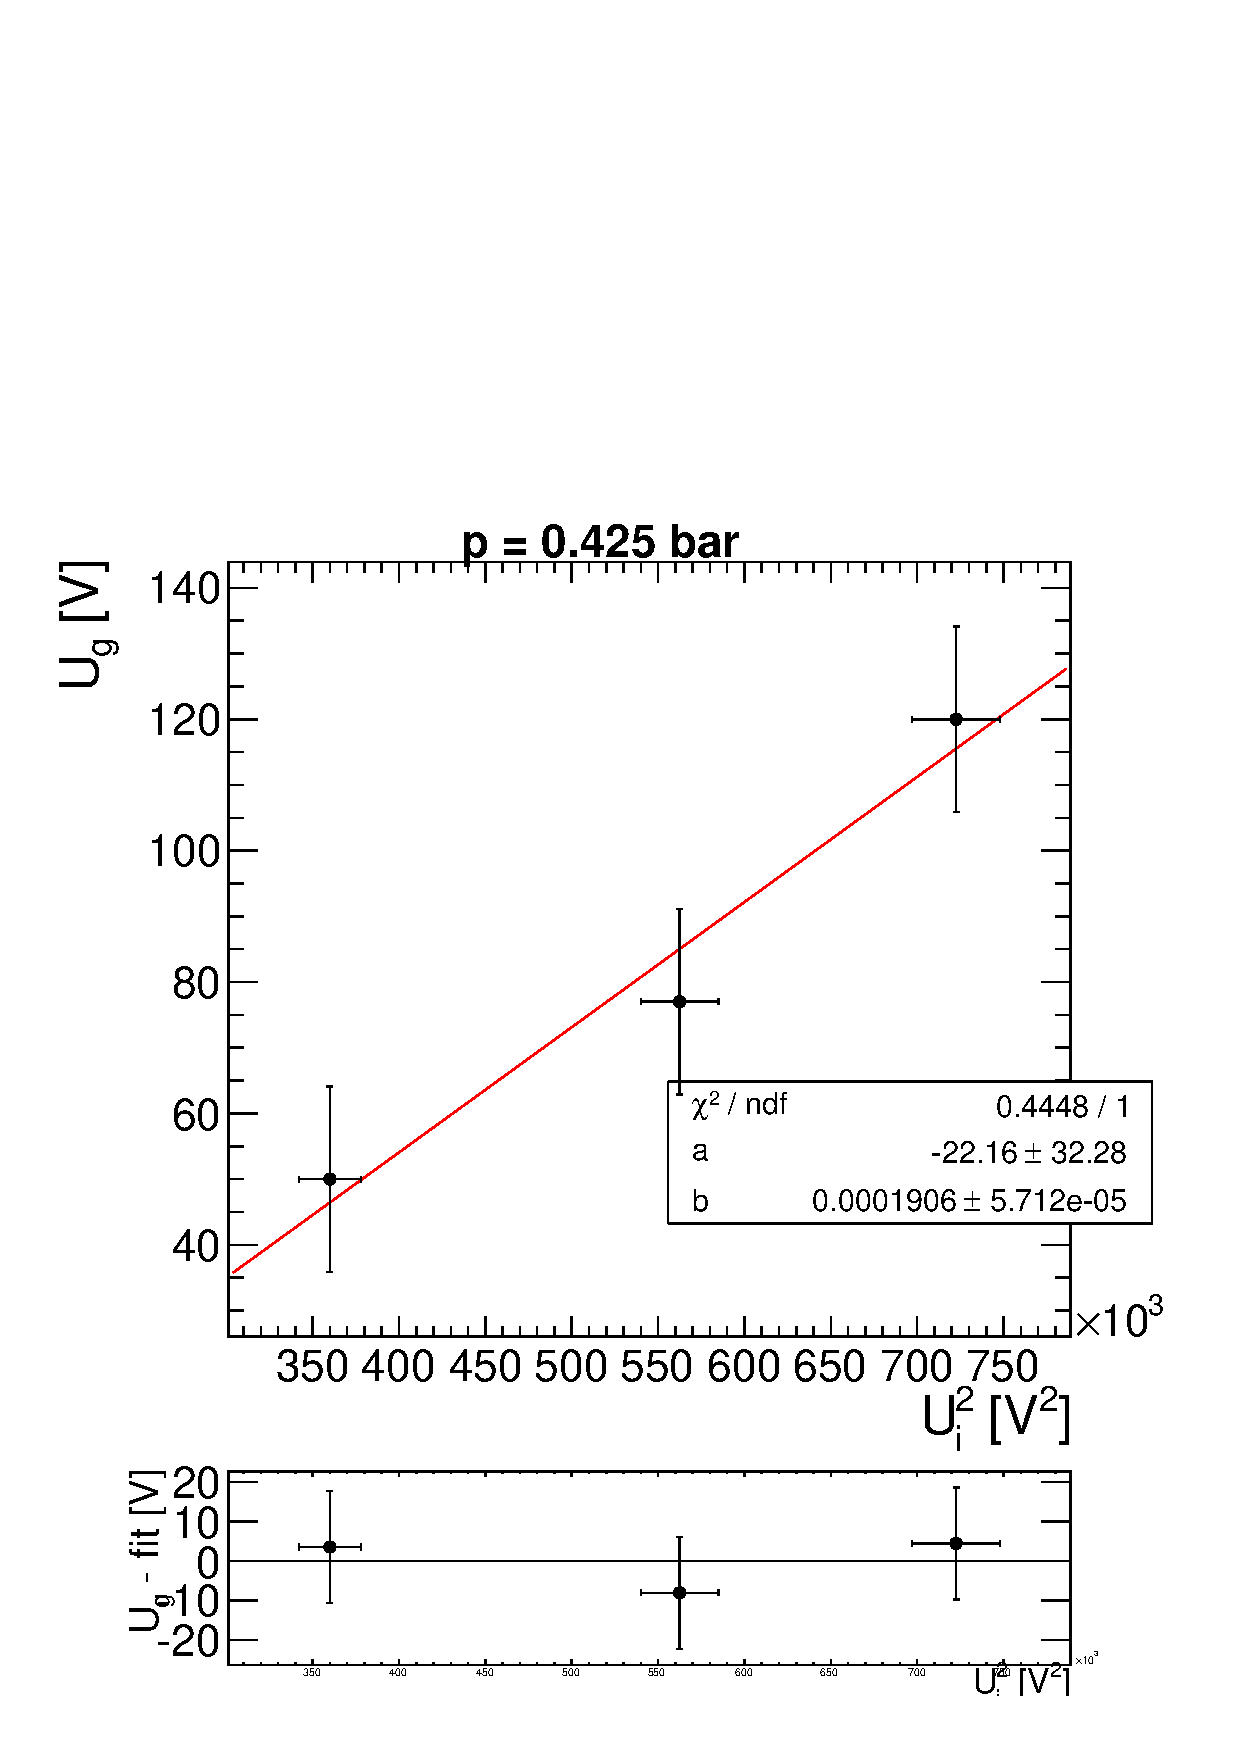
\includegraphics[height = 0.3\textheight]{linReg425bar.pdf}
		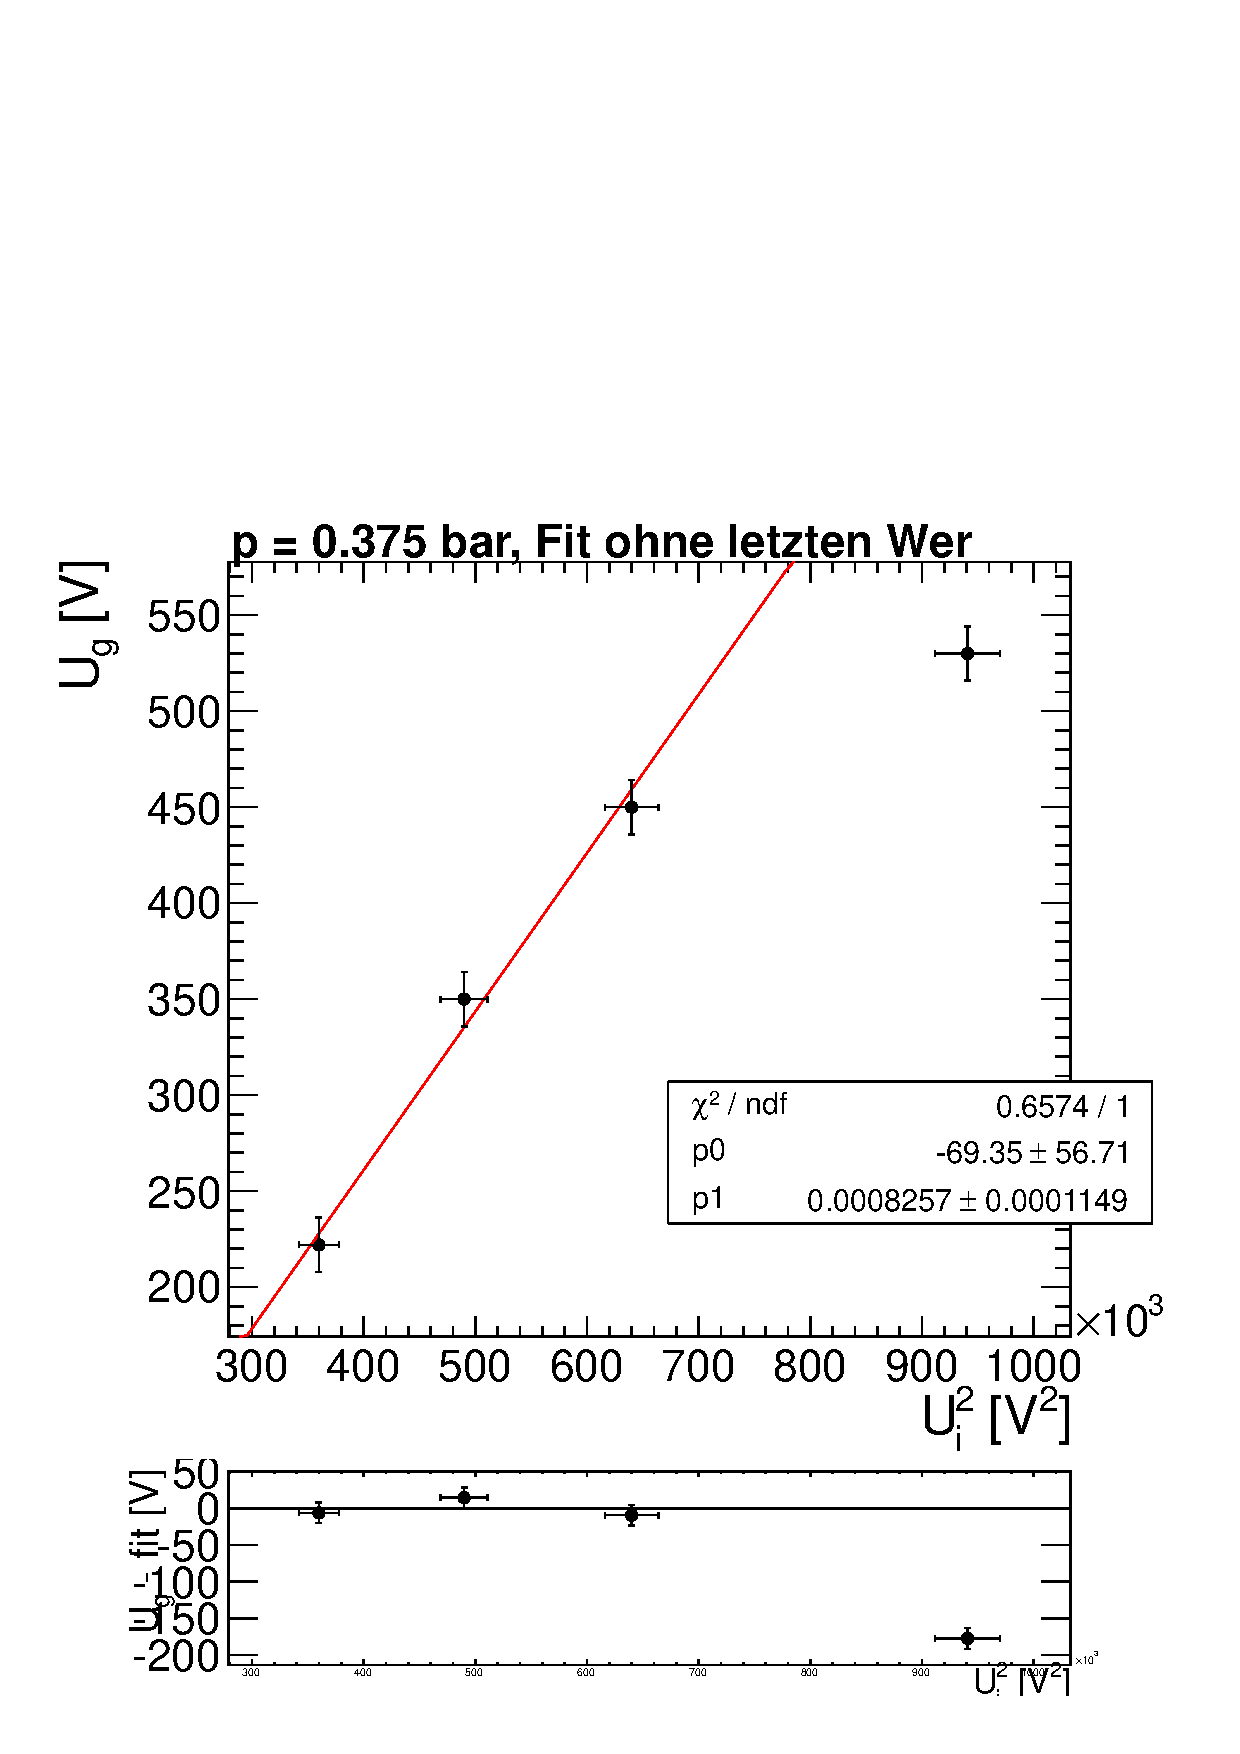
\includegraphics[height = 0.3\textheight]{linReg375bar.pdf}
		\caption{Lineare Regressionen und Residuen zur Stabilitätsuntersuchung für unterschiedliche Luftdrücke und Teilchen.
			Oben links wird der letzte Datenpunkt nicht für die Anpassung benutzt, da das Teilchen die Falle schon verlassen hat.
			Unten rechts wurde die maximale Spannung erreicht, ohne das die Stabilitätsgrenze erreicht wurde.
		}
		\label{linReg}
\end{figure}

Da der Luftdrucksensor nur $\unit[50]{mbar}$ auflösen konnte, sind die Druckangaben mit einem Fehler von $\unit[14]{mbar}$ behaftet.
Für Messungen, bei denen die Druckanzeige geschwankt hat, wurde der Mittelwert aus beiden Drücken genommen.


Für $U_i$ wird ein Fehler von $\unit[14]{V}$ verwendet, für die Gleichspannung ein Fehler von $\unit[15]{V}$, da sie nicht nur schwankt, sondern auch nur ein geringer Zeitraum zum Ablesen bestand, da die Teilchen die Falle schnell verlassen.

In der Anpassung unten rechts wird der letzte Datenpunkt nicht verwendet, da hier die Maximale Amplitude der Gleichspannung erreicht wurde.
Das eigentliche Verlassen des Stabilitätsbereichs findet bei einer höheren Spannung statt.
Da durch den genaueren Aufbau der Vakuumfalle besonders viele Teilchen gefangen werden, müssen am Anfang viele Teichen aus dem Stabilitätsbereich gebracht werden, damit man die Teichen auseinander halten kann.
Dies führt dazu, dass man nur noch sehr stabile Teilchen in der Falle hat, mit denen man schnell das Maximum der Gleichspannung erreicht.

Zugleich möchte man aber auch über das ganze Spektrum der Gleichspannung, da bei niedrigen Spannungen der relative Fehler und damit auch die Fehler auf die Anpassungsergebnisse steigen, was man oben rechts in der Abbildung sehen kann.


In der Anpassung oben links wird der letzte Datenpunkt nicht für die Anpassung verwendet, weil bei dem Punkt das Teichen schon entkommen war.
Man kann über den Abstand des letzen Punktes zur Anpassungsgerade die Spannung abschätzen die nötig gewesen wäre, ein Teichen tatsächlich aus der Falle zu bringen.
Dies spiegelt sich auch im y-Achsenabschnitt wieder, der im gewichteten Mittel $-\unit[57]{V}$ beträgt und damit mit dem Abstand zur Anpassungsgeraden konsistent ist.
% noch mehr text dazu?
Durch die lineare Regression kann also der systematische Fehler durch das konservative Abschätzen der Entweichspannung verringert werden.


Das $χ^2/ndf$ ist etwas zu klein, besonders an den Graphen, die nur Messwerte bei niedrige Gleichspannung beinhalten, da wie oben beschrieben der relative Fehler hier größer wird.
Die Fehler wurden also zu konservativ abgeschätzt.
Insgesamt sind die Anpassungen gut mit einer Geraden vereinbar.


Über die Steigung $b$ kann nun das Verhältnis von Ladung zu Masse ausgerechnet werden:
\begin{align*}
	U_G = -\frac{3K}{2Ω^2r_0^2}\frac{q}{m} U_x^2 =: b U_x^2
\end{align*}

\begin{align*}
	\Leftrightarrow \frac{q}{m} = -\frac{2Ωºr_0² b}{3K}.
\end{align*}
Die Ergebnisse sind in Tabelle \ref{tab:stabil-result} eingetragen.
In den statistischen Fehler geht der Fehler der Steigung ein, in den systematischen die Unsicherheiten von $Ω$ und $r_0$.
Der Hauptanteil des systematischen Fehlers kommt von der niedrigen Frequnez, mit der der Versuch betrieben wird.
Bei höheren Frequenzen wäre der relative Fehler kleiner, dafür wäre es schwieriger, Teilchen zu fangen.

\begin{table}[h]
	\centering
	\begin{tabular}{ c| c }
		Druck [mbar] & $\mathbf{-\frac{q}{m}[\frac{\mu C}{kg}]}$ \\
		\hline
		1000 & 201 ± 20 (stat) ± 14 (sys)\\
		1000 & 39.9 ± 27 (stat) ± 2.7 (sys)\\
		375 & 569 ± 79 (stat) ± 39 (sys)\\
		400 & 637 ± 75 (stat) ± 43 (sys)\\
		425 & 131 ± 39 (stat) ± 8.9 (sys)\\
		425 & 509 ± 31 (stat) ± 35 (sys)
	\end{tabular}
\caption{Das Verhältnis von Ladung zu Masse von verschiedenen Teichen, bestimmt durch die Stabilitätsgrenze}
\label{tab:stabil-result}
\end{table}

Man sieht keinen Zusammenhang zwischen Druck und dem Verhältnisses von Ladung zu Masse, was daran liegt, dass der Druck nicht niedrig genug war.
Auch die Werte bei gleichen oder ähnlichen Drücken sind nicht vereinbar, was damit zu erklären ist, dass die Ladung oder die Masse nicht genau festgelegt ist.




\section{Vergleich der Messungen}
Die drei genutzten Messmethoden liefern im Rahmen ihrer Fehler inkompatible Ergebnisse. Die Messwerte für $\frac{q}{m}$ unterscheiden sich deutlich um mehrere Größenordnungen:
\begin{table}[h]
	\centering
	\begin{tabular}{lr}
		Z Kompensation  & $\approx \unitfrac[ 1 ]{mC}{kg}$\\
		Resonanz & $\approx \unitfrac[ 0.1 ]{mC}{kg}$\\
		Stabilität &  $\approx \unitfrac[ 0.001-0.01 ]{mC}{kg}$\\
	\end{tabular}
	\label{result_compare}
\end{table}
%Mögliche Gründe ?
Es ist dabei zu beachten, dass die einzelnen Messungen, die mit einer Messmethode durchgeführt wurden, innerhalb ihrer Fehler
mit einander kompatibel sind.
Für die beobachteten Unterschiede gibt es zunächst zwei Erklärungsansätzte:
Entweder befinden sich alle Teilchen in einem begrenzten $\frac{q}{m}$ Bereich und nur eine Methode liefert 
richtige Ergebnisse oder die möglichen Werte für $\frac{q}{m}$ erstrecken sich über viele Größenordnungen
und jede einzelne Methode eignet sich nur dafür Teilchen aus einem bestimmten Bereich zu vermessen.
Gegen die zweite Hypothese spricht, dass sich die Teilchen im allgemeinen auch bei ausgeschalteter Gleich bzw. Wechselspannung in ihrer 
Leuchtkraft und dem Verhalten ihrer Bahn unter veränderung der Fokussierspannung stark ähneln. 
sind große Differenzen in $\frac{q}{m}$ unwahrscheinlich. 

Eine Zusammenfassung aller Ergebnisse ist in Abbildung \ref{final_plot} dargestellt ( man beachte die Überhöhung der dargestellten Fehler mit einem Faktor von 3).
\begin{figure}[htb]
		\centering
		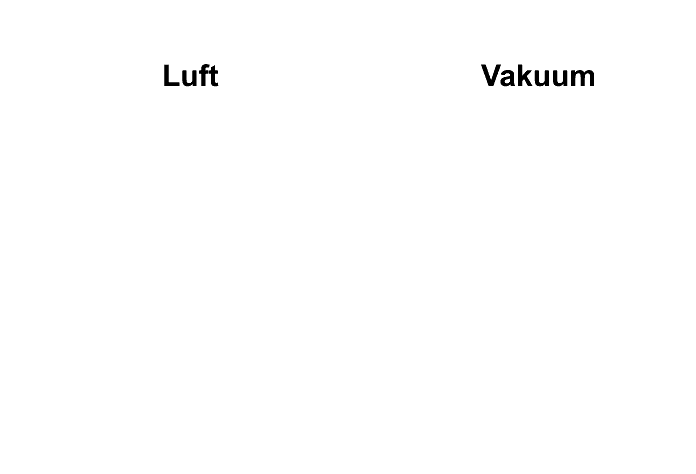
\includegraphics[height = 0.8\textwidth]{../analyse/final_plot.pdf}\\
		\caption{Zusammenfassung der Ergebnisse in logarithmische Auftragung, die Darstellung der Fehler für Stabilität und Resonanz wurden mit 3 multipliziert}
		\label{final_plot}
\end{figure}



\section{Fazit}
Die Versuchsdurchführung war dadurch geprägt das die Spannungsquelle nur stark schwankende Ausgangsspannungen geliefert hat. Besonders ein reglemäßiges plötliches Abfallen der Fokussierspannung für ein 
Flächenpaar hat zu regelmäßigem Verlust der Teilchen geführt. Insbesondere die Resonanzmessung und die Stabiliätsmessung waren oft nicht durchzuführen, weil ein langfristiges einfangen der Teilchen nicht
möglich war.

% max 30 seiten
\end{document}
